


\subsection{Challenges}
Measuring the context switch time in serverless functions has several challenges:
\begin{itemize}
	\item [C1] Characteristics of context switch in serverless environments
	
	Context switch is triggered differently in serverless functions compared to in traditional operating systems as it's scheduled by the cloud provider.
	And the service provider has the tendency to trigger more functions in the same hardware to get more profits. 
	Thus, context switch may happen not only due to performance factors like multi-threading/processing, but also provider's profit considerations.
	Besides, in Linux setting, the context switch time is related to the number of processes/threads and process/thread size. 
	In the case of serverless functions, it may be influenced by other factors.
	
	\item [C2] Benchmark accuracy
	
	As none of the existing benchmarks can be used in serverless environment, 
	it's challenging for us to reason about the accuracy of new benchmarks proposed.
	We also have to reason about the potential factors that might lead to variations in the measurement.
%	As no such benchmark is provided so far, we have to analyze the factors in our own benchmark that may lead to the potential variation to golden value, 
%	in order to reason about the accuracy of the measurement.
	% Variations to golden values in measurement 
\end{itemize}

\subsection{Context switches in serverless environment}
	In a cloud setting, the cloud provider will allocate multiple users to share the same physical device, in order to maximize the computing resource utilization.
	When there are multiple users co-locating at the same server, if the number of processes needed to run is larger than the cores inside the server, it's highly likely that there will be context switches. 
	
	Figure\ref{fig:cloud} shows one example scenario. Suppose there are two cores in a physical machine, but there are three processes need to run. 
	Each process belongs to one user. When process 1 is executing on core 1 and process 3 is executing on core 2, 
	No resource is available for process 2. In order to handle the request from process 2 simultaneously, the scheduler may interrupt process 1 and assign process 2 to run in Core 1 by saving the context register of process 1, stopping it, and restoring the registers of process 2 and start running it. 
	After a while, it switches back to process 1. In this scenario, two context switches happen and add extra execution time to process 1. 

	To tackle \emph{C1}, we design the following experiments to analyze the factors influencing context switch in serverless environments.
	% We measure the context switch execution time elapse between two adjacent lines of code repeatedly under different configurations in serverless functions.
	Shahrad \emph{et al.} \cite{serverless-main} shows that the execution time in serverless functions is influenced by function invocation frequency, memory size and function execution time.
	Since invocation frequency only influences the time that the function is called and has no impact on the execution process of the function itself,
	we choose to observe the context switch time under different memory size and function execution time setting.
	Recall that in Table \ref{tab:price} with more memory allocated, the function will enjoy higher CPU frequency and thus more CPU computing resources, 
	which might influence the amount of context switches during the function execution.
	


	% Theoretically, the measured time elapse should be 0 as there is no execution between these two lines. 
	% However, our initial experiments show that this is neither 0 nor a fixed value, indicating that interruption happens between these two lines
	% and the time elapse changes with different configurations. 
	% Although the interruption is not limited to context switch but also page faults handling or container management, 
	% it can still provide insights in the influence of different configurations on context switch time in serverless environments.


\subsection{Combine various benchmarks}
	To tackle \emph{C2}, we first run our own designed benchmarks on local Linux system and compare the results with published benchmarks\cite{cs-lmbench,cs-pipes,cs-arm,cs-web},
	 ensuring the correctness of the proposed ones. Then we deploy the new benchmarks in serverless functions and compare the results. 
	 If one of the benchmarks is consistently higher or lower than others, then we'll explore the reasons and this can help us improve our accuracy.
	% Currently, the new benchmarks are designed as the prior benchmarks with different configurations.
	The prior benchmarks we are choosing are:
	
	1. Pingpong pipes\cite{cs-pipes,cs-web}: In Fig.\ref{fig:pipes}, two threads or processes are created and pinned to a single core. 
		      One thread writes the data to another thread through a pipe, which induces a context switch. 
			  After the data is read, the read thread transfers the data to write thread/process and this induces another context switch.
			  The total execution time equals the read and write operation time adds two context switch time.
			  In contrast, a single thread and two pipes are created. It passes the data through a pipe to itself. 
			  Here the total execution time only consists of the read and write operation time.
			  By subtracting these two time and dividing the result with 2, we get the thread context switch time.
	
	2. Condition var\cite{cs-web}: A shared variable between two threads is used and is protected by mutex to prevent it from being modified by two threads at the same time.
		      A signal is passed between two threads to tell which thread has the access to write the variable.
			  And by passing the signals, the context will switch from one thread to the other. 
			  The time for the signal changes is the context switch time.
	
	3.  Lmbench\cite{cs-lmbench}: A ring of pipes is created, and a token is passed from process to process with these pipes. 
	          Also, the time of passing the token in a single process with this ring of pipes is measured. 
			  Subtraction of these two time is the total context switch time of a number of context switches.

\subsection{Benchmarks in serverless environment}
	The aforementioned benchmarks can't be directly applied to serverless environment as they were all written in C.
	However, most mainstream serverless functions only support programming languages including Python, Java, Ruby and Go.
	In this project, we choose to write own benchmarks in Python.

	Context switches can be divided into thread context switch and process context switch. 
	\textbf{Thread context switch}

	This design is similar to \emph{Pingpong pipes}\cite*{cs-pipes,cs-web} in Section 2.3, 
	the only difference that we made is we rewrote the algorithm from C language to Python.

	\textbf{Process context switch}

	This design is similar to \emph{Lmbench}\cite{cs-lmbench}. 
	However, we add modifications to the original algorithm to make it more self-explainable.
	In Fig.\ref{fig:ring}, a ring of processes is created and pinned to a single core. 
	Each two of them are connected with a pipe. 
	The parent process will pass its process id(PID) to next process. 
	Process 2 reads the PID through the pipe, add it with its own PID, then write the new PID sum into the next pipe. 
	For the following processes, it will read the sum of previous PIDs, add it with itself, and pass the new sum to next process. 
	At last, the parent process will read the sum of all PIDs from the last pipe. 
	The benefit of this design is, by checking the last value read by Process 1 with sum of PIDs, we can ensure that the value is passed through pipes. 
	This design also enables us to analyze if the number of processes will affect the context switch time.
	As for the baseline, N pipes and 1 process are created to measure the read and write time. 
	The result for subtracting T1 with T2 is the time for N context switches.
	
\begin{figure}
	\centering
	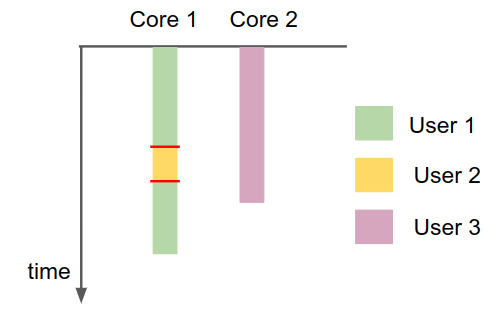
\includegraphics[width=\linewidth]{./figure/cxt_cloud.png}
	\caption{Context switches in serverless computing}
	\label{fig:cloud}
\end{figure}

\begin{figure}
	\centering
	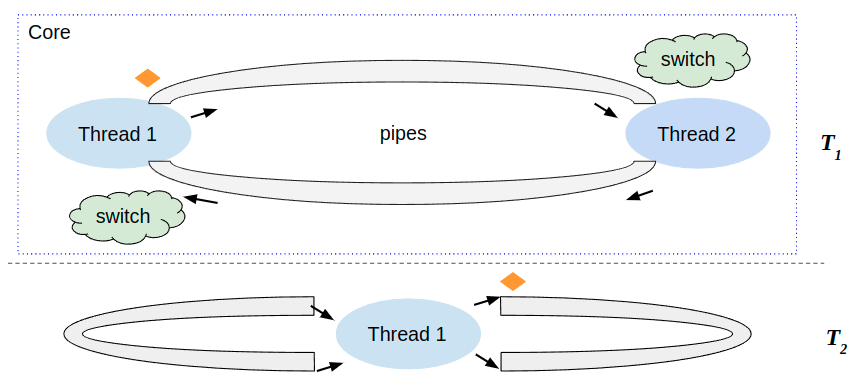
\includegraphics[width=\linewidth]{./figure/pipes.png}
	\caption{Measuring thread context switches with two pipes}
	\label{fig:pipes}
\end{figure}

\begin{figure}
	\centering
	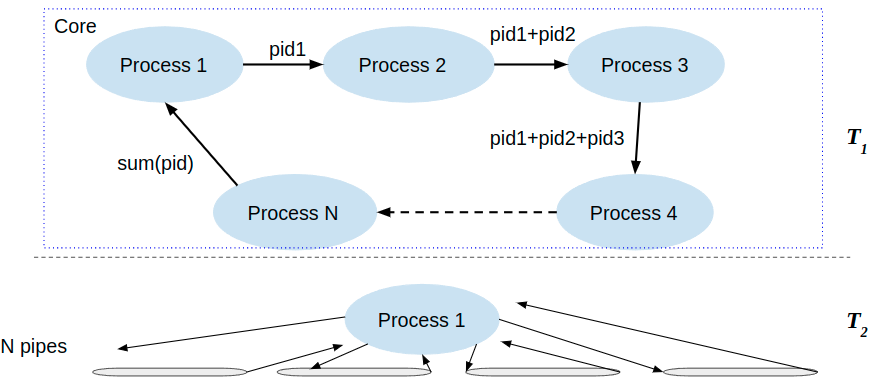
\includegraphics[width=\linewidth]{./figure/ring.png}
	\caption{Measuring process context switches with ring pipes}
	\label{fig:ring}
\end{figure}

% "Based on these traditional methods, we also used pipe communication to implement frequent context switches between two processes."
